% Options for packages loaded elsewhere
\PassOptionsToPackage{unicode}{hyperref}
\PassOptionsToPackage{hyphens}{url}
%
\documentclass[
]{article}
\usepackage{lmodern}
\usepackage{amsmath}
\usepackage{ifxetex,ifluatex}
\ifnum 0\ifxetex 1\fi\ifluatex 1\fi=0 % if pdftex
  \usepackage[T1]{fontenc}
  \usepackage[utf8]{inputenc}
  \usepackage{textcomp} % provide euro and other symbols
  \usepackage{amssymb}
\else % if luatex or xetex
  \usepackage{unicode-math}
  \defaultfontfeatures{Scale=MatchLowercase}
  \defaultfontfeatures[\rmfamily]{Ligatures=TeX,Scale=1}
\fi
% Use upquote if available, for straight quotes in verbatim environments
\IfFileExists{upquote.sty}{\usepackage{upquote}}{}
\IfFileExists{microtype.sty}{% use microtype if available
  \usepackage[]{microtype}
  \UseMicrotypeSet[protrusion]{basicmath} % disable protrusion for tt fonts
}{}
\makeatletter
\@ifundefined{KOMAClassName}{% if non-KOMA class
  \IfFileExists{parskip.sty}{%
    \usepackage{parskip}
  }{% else
    \setlength{\parindent}{0pt}
    \setlength{\parskip}{6pt plus 2pt minus 1pt}}
}{% if KOMA class
  \KOMAoptions{parskip=half}}
\makeatother
\usepackage{xcolor}
\IfFileExists{xurl.sty}{\usepackage{xurl}}{} % add URL line breaks if available
\IfFileExists{bookmark.sty}{\usepackage{bookmark}}{\usepackage{hyperref}}
\hypersetup{
  pdftitle={Write Up},
  pdfauthor={Louis Condevaux},
  hidelinks,
  pdfcreator={LaTeX via pandoc}}
\urlstyle{same} % disable monospaced font for URLs
\usepackage[margin=1in]{geometry}
\usepackage{graphicx}
\makeatletter
\def\maxwidth{\ifdim\Gin@nat@width>\linewidth\linewidth\else\Gin@nat@width\fi}
\def\maxheight{\ifdim\Gin@nat@height>\textheight\textheight\else\Gin@nat@height\fi}
\makeatother
% Scale images if necessary, so that they will not overflow the page
% margins by default, and it is still possible to overwrite the defaults
% using explicit options in \includegraphics[width, height, ...]{}
\setkeys{Gin}{width=\maxwidth,height=\maxheight,keepaspectratio}
% Set default figure placement to htbp
\makeatletter
\def\fps@figure{htbp}
\makeatother
\setlength{\emergencystretch}{3em} % prevent overfull lines
\providecommand{\tightlist}{%
  \setlength{\itemsep}{0pt}\setlength{\parskip}{0pt}}
\setcounter{secnumdepth}{-\maxdimen} % remove section numbering
\ifluatex
  \usepackage{selnolig}  % disable illegal ligatures
\fi

\title{Write Up}
\author{Louis Condevaux}
\date{12/15/2020}

\begin{document}
\maketitle

\section*{Introduction}

After struggling quite a bit with R Markdown. Here is my final write up.
Aim training is an essential basis of most video games that include any
type of fighting mechanic that are not assisted by any software. It may
range from moving your mouse and click at the right time on the target
or simply follow the target for a specific amount of time. These
scenarios are supposed to recreate the type of action you may encounter
in some games to focus on your weaknesses or simply to get better at in
an area. In theory, aim trainers are supposed to make you aim better in
different games if you create the same environment.

\subsection{History}

A lot of aim trainers have emerged during these last years with the
growing of esport and their prize pools. These games are mostly used for
first and third person shooters in which you require precise aiming in
any situation. Counter Strike Global Offensive, Overwatch, Fortnite, are
great examples of games requiring a consistent aim in which pros have
recognized using aim trainers as a form of practice. There are a lot of
aim trainers, varying from being free to around \$15.

\subsection{Kovaak}

Kovaak is the aim trainer I decided to analyze since I already bought it
before this class. Kovaak is recognized as one of the best aim trainer
due to its great number of different scenarios as well as the
customization possible by the players. It is important to be noted that
anyone can create scenarios as they wish, which helps having a wide
variety of scenarios for most of the games. There is also a possibility
to extract your data under the form of excel files. However, their
format is not great and could use some rework (as I realized).

\subsection{Player}

I thought this section could be useful to bring more light to the
results later. I started playing Kovaak on a non-consistent basis about
a year ago. I started by doing the most popular scenarios and slowly
started to follow some guides. I quickly improved at first but I was not
sure if the time put in playing it was worth the improvement. Also,
there seemed to be a lack of solid correlation between playing the aim
trainer or directly playing the main game. These two factors led to
inconsistent data over time.

\section*{Packages}

Most of the packages used for this project consisted of tools to extract
and format the data. Formatting the data was my greatest challenge
because of the way it was extracted form the game.

\begin{enumerate}
\def\labelenumi{\arabic{enumi}.}
\tightlist
\item
  data.table
\end{enumerate}

\begin{itemize}
\tightlist
\item
  Helped with data manipulation.
\end{itemize}

\begin{enumerate}
\def\labelenumi{\arabic{enumi}.}
\setcounter{enumi}{1}
\tightlist
\item
  dplyr
\end{enumerate}

\begin{itemize}
\tightlist
\item
  Helped with data manipulation.
\end{itemize}

\begin{enumerate}
\def\labelenumi{\arabic{enumi}.}
\setcounter{enumi}{2}
\tightlist
\item
  tidyverse
\end{enumerate}

\begin{itemize}
\tightlist
\item
  Commong package that offers a lot of possibilities for data science.
\end{itemize}

\begin{enumerate}
\def\labelenumi{\arabic{enumi}.}
\setcounter{enumi}{3}
\tightlist
\item
  fs
\end{enumerate}

\begin{itemize}
\tightlist
\item
  This package was really helpful dealing with the data from my
  directory to import them into R.
\end{itemize}

\begin{enumerate}
\def\labelenumi{\arabic{enumi}.}
\setcounter{enumi}{4}
\tightlist
\item
  lubridate
\end{enumerate}

\begin{itemize}
\tightlist
\item
  Helped with date formatting.
\end{itemize}

\begin{enumerate}
\def\labelenumi{\arabic{enumi}.}
\setcounter{enumi}{5}
\tightlist
\item
  sqldf
\end{enumerate}

\begin{itemize}
\tightlist
\item
  Sqldf is the only one that is a bit different from the others. It is
  used to take advantage of the SQL language and syntax. This package
  helped my code to be clearer and more understandable by using tables
  names.
\end{itemize}

\begin{enumerate}
\def\labelenumi{\arabic{enumi}.}
\setcounter{enumi}{6}
\tightlist
\item
  magrittr
\end{enumerate}

\begin{itemize}
\tightlist
\item
  Used mainly for the pipe operator
\end{itemize}

\begin{enumerate}
\def\labelenumi{\arabic{enumi}.}
\setcounter{enumi}{7}
\tightlist
\item
  ggpubr
\end{enumerate}

\begin{itemize}
\tightlist
\item
  Used to add ggplots on the same layout.
\end{itemize}

\section*{Visualization}

\begin{figure}
\centering
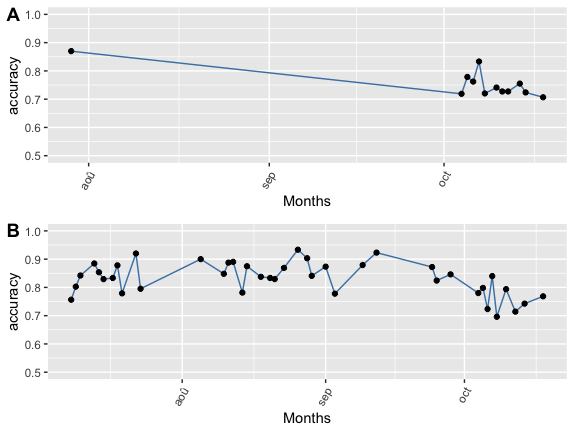
\includegraphics{/Users/Louis/Desktop/CADS/510/Midterm/Pictures/both_plots.png}
\caption{Both Graphs}
\end{figure}

\subsection{Graph 1}

\begin{figure}
\centering
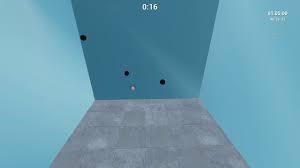
\includegraphics{/Users/Louis/Desktop/CADS/510/Midterm/Pictures/one_wall_ex.jpg}
\caption{Bounce Scenario Example}
\end{figure}

To bring more context, the ``one wall five targets pasu'' scenario is
considered to be an intermediate/advanced scenario. It requires
``clicking'' and ``tracking'' to get a good score. To get a score, you
need to click on as many targets as possible during a minute. These
targets move midly fast on the rectangle grid in random direction.
Therefore, to get a good score, you need to anticipate the trajectory of
the target as well as tracking it at the same time. You also need to be
able to switch fast between targets.

\begin{figure}
\centering
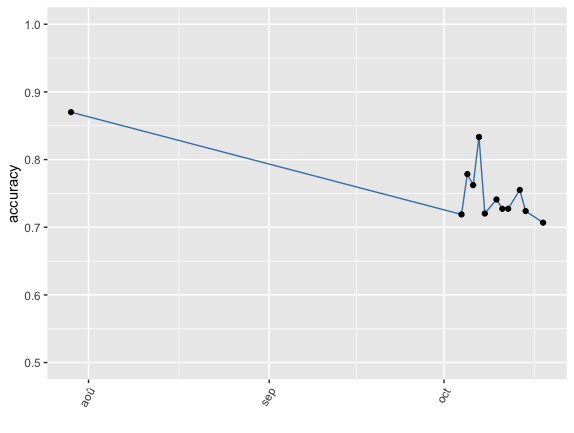
\includegraphics{/Users/Louis/Desktop/CADS/510/Midterm/Pictures/one_wall.png}
\caption{One Wall Scenario Over 5 Months}
\end{figure}

This graph shows that not only it lacks data over time but also that
there does not seem to be a real progression. As stated previously in
the ``Player'' section, I started to play this scenario less because I
either wasn't training my aim anymore or that I started playing
different scenarios. Other reasons affected the results but I will
discuss it in another section.

\subsection{Graph 2}

\begin{figure}
\centering
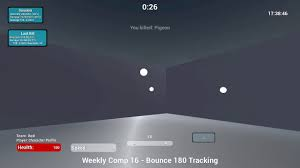
\includegraphics{/Users/Louis/Desktop/CADS/510/Midterm/Pictures/bounce_ex.jpg}
\caption{Bounce Scenario Example}
\end{figure}

The bounce scenario differs from the previous one because of the space
the balls can go as well as the field of view. This scenario is also
considered as intermediate and focuses more on tracking since the balls
do not go as fast and follow the same pattern. The place they spawn is
what will determine their trajectory but you also may need to react fast
since they can collide into each others.

\begin{figure}
\centering
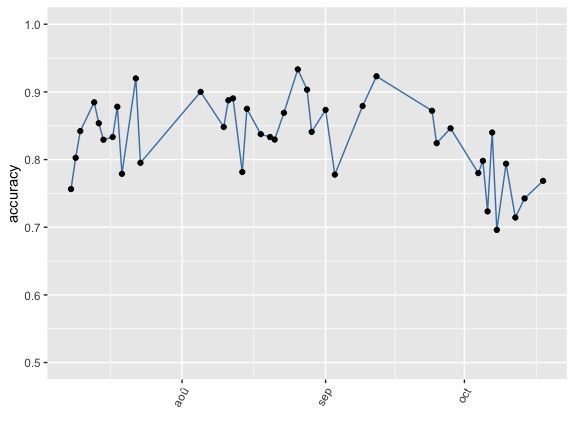
\includegraphics{/Users/Louis/Desktop/CADS/510/Midterm/Pictures/Bounce_scenario.png}
\caption{Bounce Scenario Over 5 Months}
\end{figure}

As seen on the graph, I played this scenario way more consistenly than
the last one. However, there does not seem to show progression, but
instead the opposite. However, the results can still be considered as
correct since the accuracy did not go below 70\% as a whole.

\subsection*{Data Visualization Summary}

Both of these graphs did not show any kind of constant progression over
time. A few reasons could explain these somewhat inconsistent results.
Extraneous variables played a big role in the results such as the time
the scenario was played (i.e, morning vs afternoon), the difficulty of
the scenario, the position it was played (i.e, use of guides), as well
as the number of times played in a row. All of these reasons focus more
on the routine of the player and may affect the results. We could also
include what is called the ``plateau effect.'' Moreover, any hardware
change could greatly influence the results such as a changing a mouse,
monitor etc\ldots{} Finally, it is indeed really hard to create some
baseline to measure progression over time and keep each variable the
same. The player may feel the need to change some of these to acquire
more comfort or because he may think the change will show a greater
progression over time.

\section*{Summary}

This project was quite difficult for reasons that I did not expect. I
have never been realy familiar with R and especially doing data
transformation in R. I guess it was the perfect data set to explore
because of the way it was constructed and what I had to do to make it
fit what I expected it to be. Unfortunately, I could not get rid of the
formatting errors in the tables that you specified. Overall, adding all
these little parts together was fun and I learnt a lot. Obviously, there
is a lot of room for improvement especially since I have been stupid
enough to not commit to git and made Rstudio crash on me erasing my
progression (lesson learnt!).

\subsection*{Future}

I hope that I will find a better way to collect data either from this
aim trainer or another to avoid loosing that much. This would greatly
help to create better functions and make it more accessible to others.
Still thinking of adding new games.

\end{document}
